\documentclass[12pt]{article}
\linespread{1.3}
\usepackage{hyperref}
\usepackage{enumitem}
%\usepackage{enumerate}
\usepackage{changepage,lipsum,titlesec, longtable}
\usepackage{cite}
\usepackage{comment, xcolor}
\usepackage[pdftex]{graphicx}
  \graphicspath{{images/}, {images/stat/}}
  \DeclareGraphicsExtensions{.pdf,.jpeg,.png, .jpg}
\usepackage[cmex10]{amsmath}
\usepackage{tikz}
\usepackage{array} 
\usepackage{subfigure} 
\newcommand{\grey}[1]{\textcolor{black!30}{#1}}
\newcommand{\red}[1]{\textcolor{red!50}{#1}}
\newcommand{\question}[1]{\textcolor{magenta}{\textbf{Question: } {#1}}}
\newcommand{\fref}[1]{Figure~\ref{#1}}
\newcommand{\tref}[1]{Table~\ref{#1}}
\newcommand{\eref}[1]{Equation~\ref{#1}}
\newcommand{\cref}[1]{Chapter~\ref{#1}}
\newcommand{\sref}[1]{Section~\ref{#1}}
\newcommand{\aref}[1]{Appendix~\ref{#1}}

\renewcommand{\labelenumii}{\theenumii}
\renewcommand{\theenumii}{\theenumi.\\arabic{enumii}.}

\oddsidemargin0cm
\topmargin-2cm %I recommend adding these three lines to increase the
\textwidth16.5cm %amount of usable space on the page (and save trees)
\textheight23.5cm

\makeatletter
\renewcommand\paragraph{\@startsection{paragraph}{4}{\z@}%
            {-2.5ex\@plus -1ex \@minus -.25ex}%
            {1.25ex \@plus .25ex}%
            {\normalfont\normalsize\bfseries}}
\makeatother
\setcounter{secnumdepth}{4} % how many sectioning levels to assign numbers to
\setcounter{tocdepth}{4}    % how many sectioning levels to show in ToC

% draw diagram
\usetikzlibrary{shapes.geometric, arrows}
\tikzstyle{data} = [font=\footnotesize, rectangle, rounded corners, minimum width=3cm, minimum height=1cm,align=left, draw=black, fill=black!30]
\tikzstyle{database} = [font=\footnotesize, rectangle, rounded corners, minimum width=3cm, minimum height=1cm,align=left, draw=black, fill=green!30]
\tikzstyle{query} = [trapezium, trapezium left angle=70, trapezium right angle=110, minimum width=3cm, minimum height=1cm, text centered, draw=black, fill=blue!30]
\tikzstyle{process} = [rectangle, minimum width=3cm, minimum height=1cm, text centered, draw=black, fill=orange!30]
\tikzstyle{spliter} = [diamond, minimum width=2cm, minimum height=1cm, text centered, draw=black, fill=green!30]
\tikzstyle{decision} = [diamond, minimum width=3cm, minimum height=1cm, text centered, draw=black, fill=green!30]
\tikzstyle{arrow} = [thick,->,>=stealth]
\tikzstyle{bi-arrow} = [thick,->,>=stealth]


\begin{document}
\title{Retrieving Building Snapshot ID\\
       \large SEED project}
\maketitle
\tableofcontents
\newpage
\section{Introduction}\label{sec:intro}
The document records the process of retrieving the building snapshot
id and canonical building id from SEED database.

\section{Outline}\label{sec:outline}
\subsection{With template excel file}
\subsubsection{Pseudo Code}
\makeatletter
\def\verbatim@font{\linespread{1}\small\ttfamily}
\begin{verbatim}
User:
Fill out the PM template table with their building information
Upload tables some remote folder (for us to download)
Upload tables to SEED database (making sure there is an ID created)

We:
Download the remote folder that contains the tables with the specified format.
For each table in the folder:
    Read the table into a data frame (Python pandas dataframe)
    //note: since the table is not uploaded to EnergyStar PM, 
    //the Portfolio Manager ID might not be available
    Get a set (dictionary key), A, of addresses from the PM table
    Create an empty dictionary D (initializing all entries to None)
        for each address a in the set A:
            make a QUERY to SEED database with (address, 
                                                Portfolio Manager ID) 
                if address identifies a building b is in SEED database
                    //SEED.BuildingSnapshot.id
                    get the building snapshot id: s_id
                    make a QUERY with s_id to get c_id
                    //SEED.BuildingSnapshot.canonical_building
                    D[a] = {buildingsnapshot_id: s_id,
                            canonical_building: c_id}
                else 
                    D[a] = None
    Insert the c_id, s_id to the dataframe
    convert the dataframe to json format
\end{verbatim}
\subsubsection{Diagram}
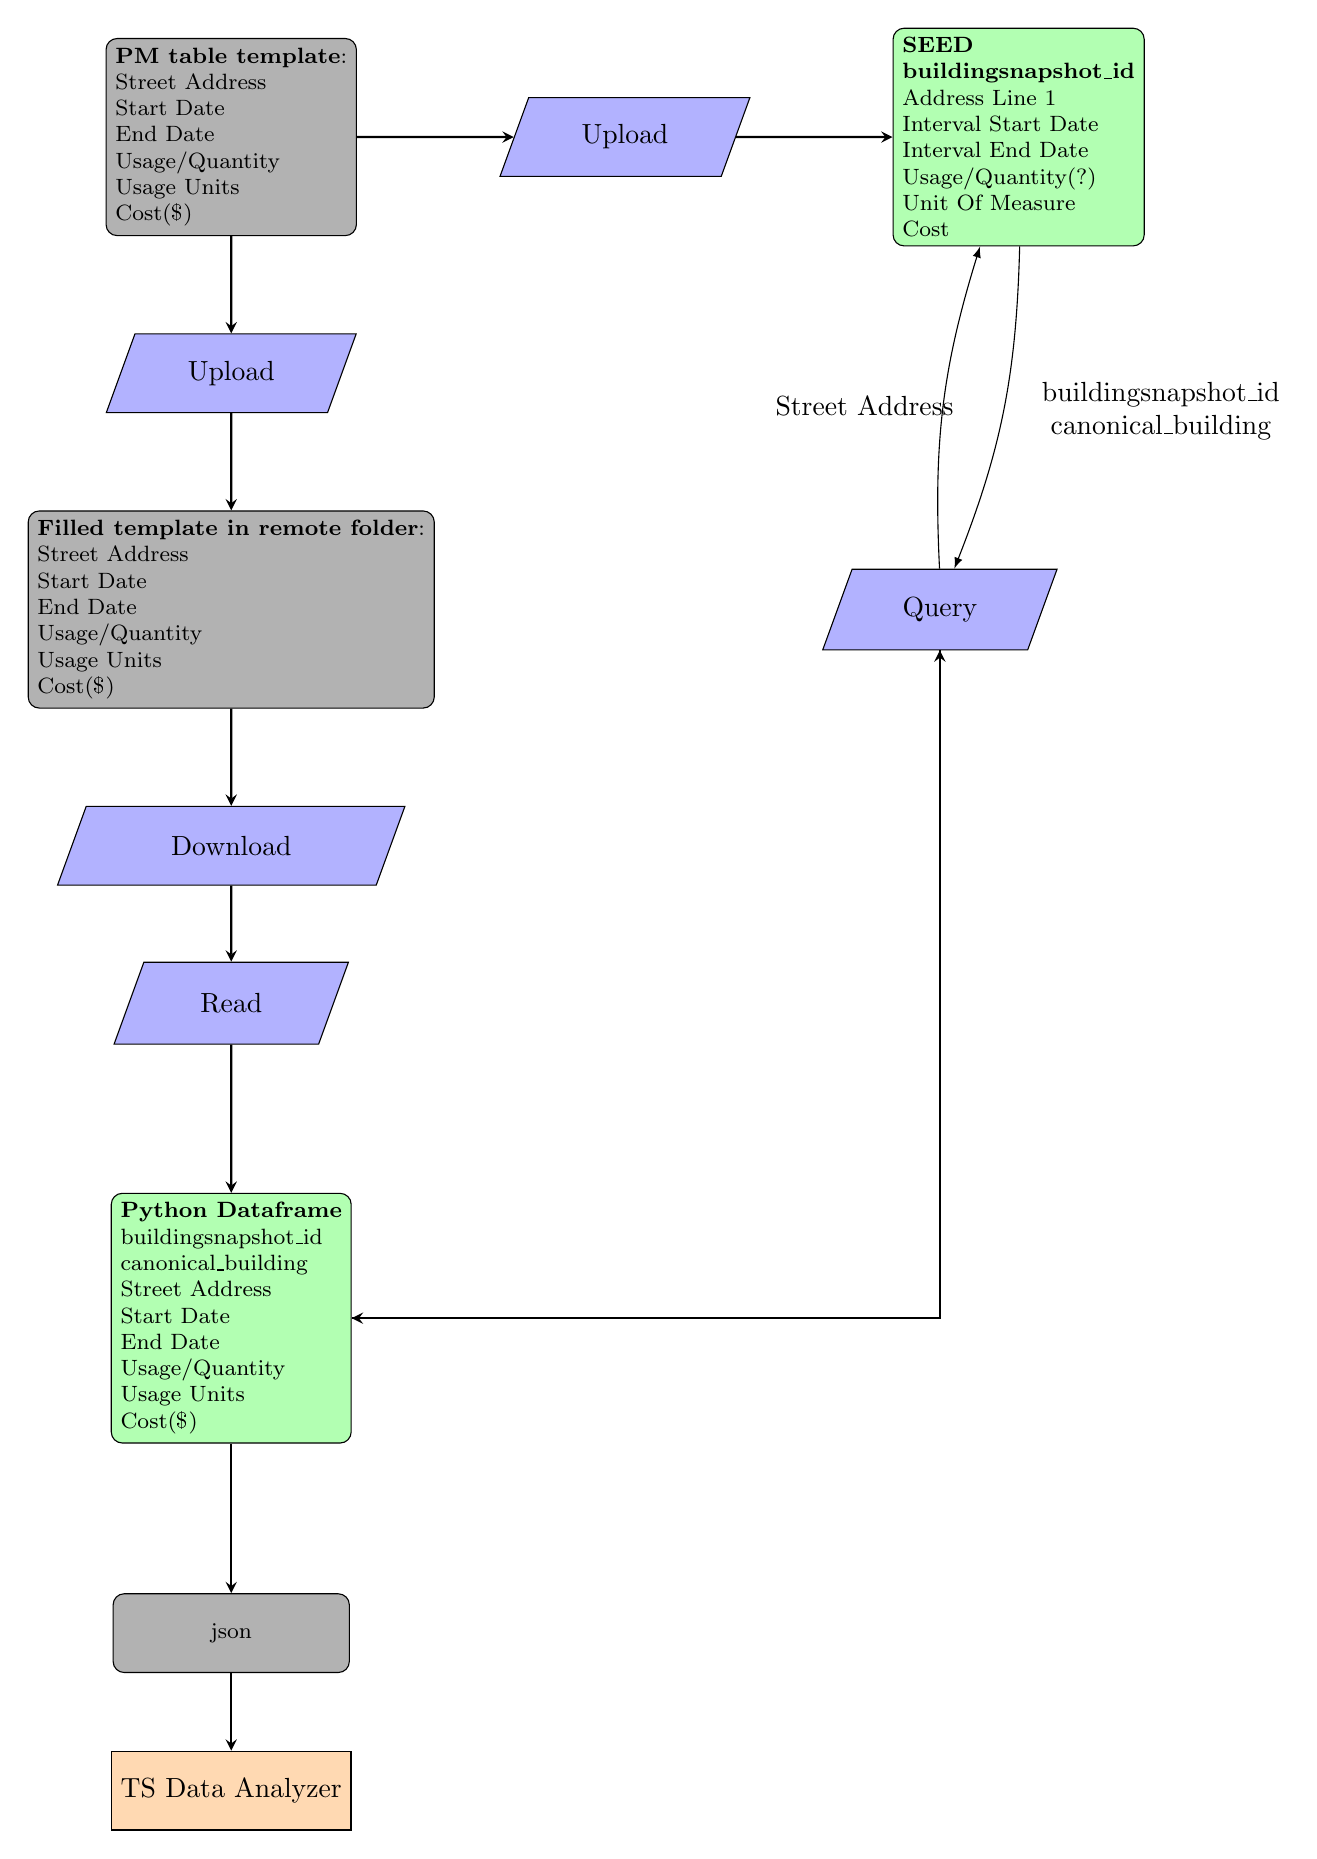
\begin{tikzpicture}
  \node (PM_table) [data]{\textbf{PM table template}:\\
    Street Address\\
    Start Date\\
    End Date\\
    Usage/Quantity\\
    Usage Units\\
    Cost(\$)};
  \node (upload)[query, right of = PM_table, xshift=4cm]{Upload};
  \node (upload2)[query, below of = PM_table, yshift=-2cm]{Upload};
  \node (SEED db)[database, right of = upload, xshift=4cm]{\textbf{SEED}\\
    \textbf{buildingsnapshot\_id}\\
    Address Line 1\\
    Interval Start Date\\
    Interval End Date\\
    Usage/Quantity(?)\\
    Unit Of Measure\\
    Cost};
  \node (remote folder) [data, below of=upload2, yshift = -2cm]{\textbf{Filled template in remote
      folder}:\\
    Street Address\\
    Start Date\\
    End Date\\
    Usage/Quantity\\
    Usage Units\\
    Cost(\$)};
  \node (download)[query, below of = remote folder, yshift=-2cm]{Download};
  \node (read)[query, below of = download, yshift=-1cm]{Read};
  \node(dataframe)[database, below of=read, yshift = -3cm]{\textbf{Python Dataframe}\\
    buildingsnapshot\_id\\
    canonical\_building \\
    Street Address\\
    Start Date\\
    End Date\\
    Usage/Quantity\\
    Usage Units\\
    Cost(\$)};
  \node(json)[data, below of=dataframe, yshift = -3cm]{json};
  \node(ext)[process, below of=json, yshift = -1cm]{TS Data Analyzer};
  \node(query)[query, right of=remote folder, xshift = 8cm]{Query};
  \draw[arrow](PM_table) -- (upload);
  \draw[arrow](upload) -- (SEED db);
  \draw[arrow](PM_table) -- (upload2);
  \draw[arrow](upload2) -- (remote folder);
  \draw[arrow](remote folder) -- (download);
  \draw[arrow](download) -- (read);
  \draw[arrow](read) -- (dataframe);
  \draw[arrow](dataframe) -| (query);
  \draw[arrow](query) |- (dataframe);
  \draw[arrow](dataframe) -- (json);
  \draw[arrow](json) -- (ext);
  %\draw[arrow, xshift = -1cm](query) -- (SEED db);
  %\draw[arrow, xshift = 1cm](SEED db) -- (query);
  \draw[-latex] (query) to[bend left=10] node [xshift=-1cm]{Street Address} (SEED
  db); 
  \draw[-latex] (SEED db) to[bend left=10] node [xshift=2cm,align=center]{buildingsnapshot\_id\\canonical\_building}
  (query);
\end{tikzpicture}

\subsection{With PM excel file}
\subsubsection{Pseudo code}
\begin{verbatim}
User:
Fill out EnergyStar PM table with their building information
Download the excel from EnergyStar
Upload tables to SEED database (making sure there is an ID created)

We:
Download the remote folder that contains the tables with the specified format.
For each table in the folder:
    Read the table into a data frame (Python pandas dataframe)
    Get a set (dictionary key), A, of ...
    (addresses, Portfolio Manager ID) pairs from the PM table
    Create an empty dictionary D (initializing all entries to None)
        for each address a in the set A:
            make a QUERY to SEED database with (address, Portfolio Manager ID) 
                if (address, Portfolio Manager ID) identifies ...
                a building b is in SEED database
                    get the building snapshot id: s_id
                    make a QUERY with s_id to get the c_id 
                    //(SEED.BuildingSnapshot.canonical_building)
                    D[a] = {buildingsnapshot_id: s_id,
                            canonical_building: c_id}
                else 
                    D[a] = None
    Insert the c_id, s_id to the dataframe
    convert the dataframe to json format
\end{verbatim}
\pagebreak
\subsubsection{Diagram}
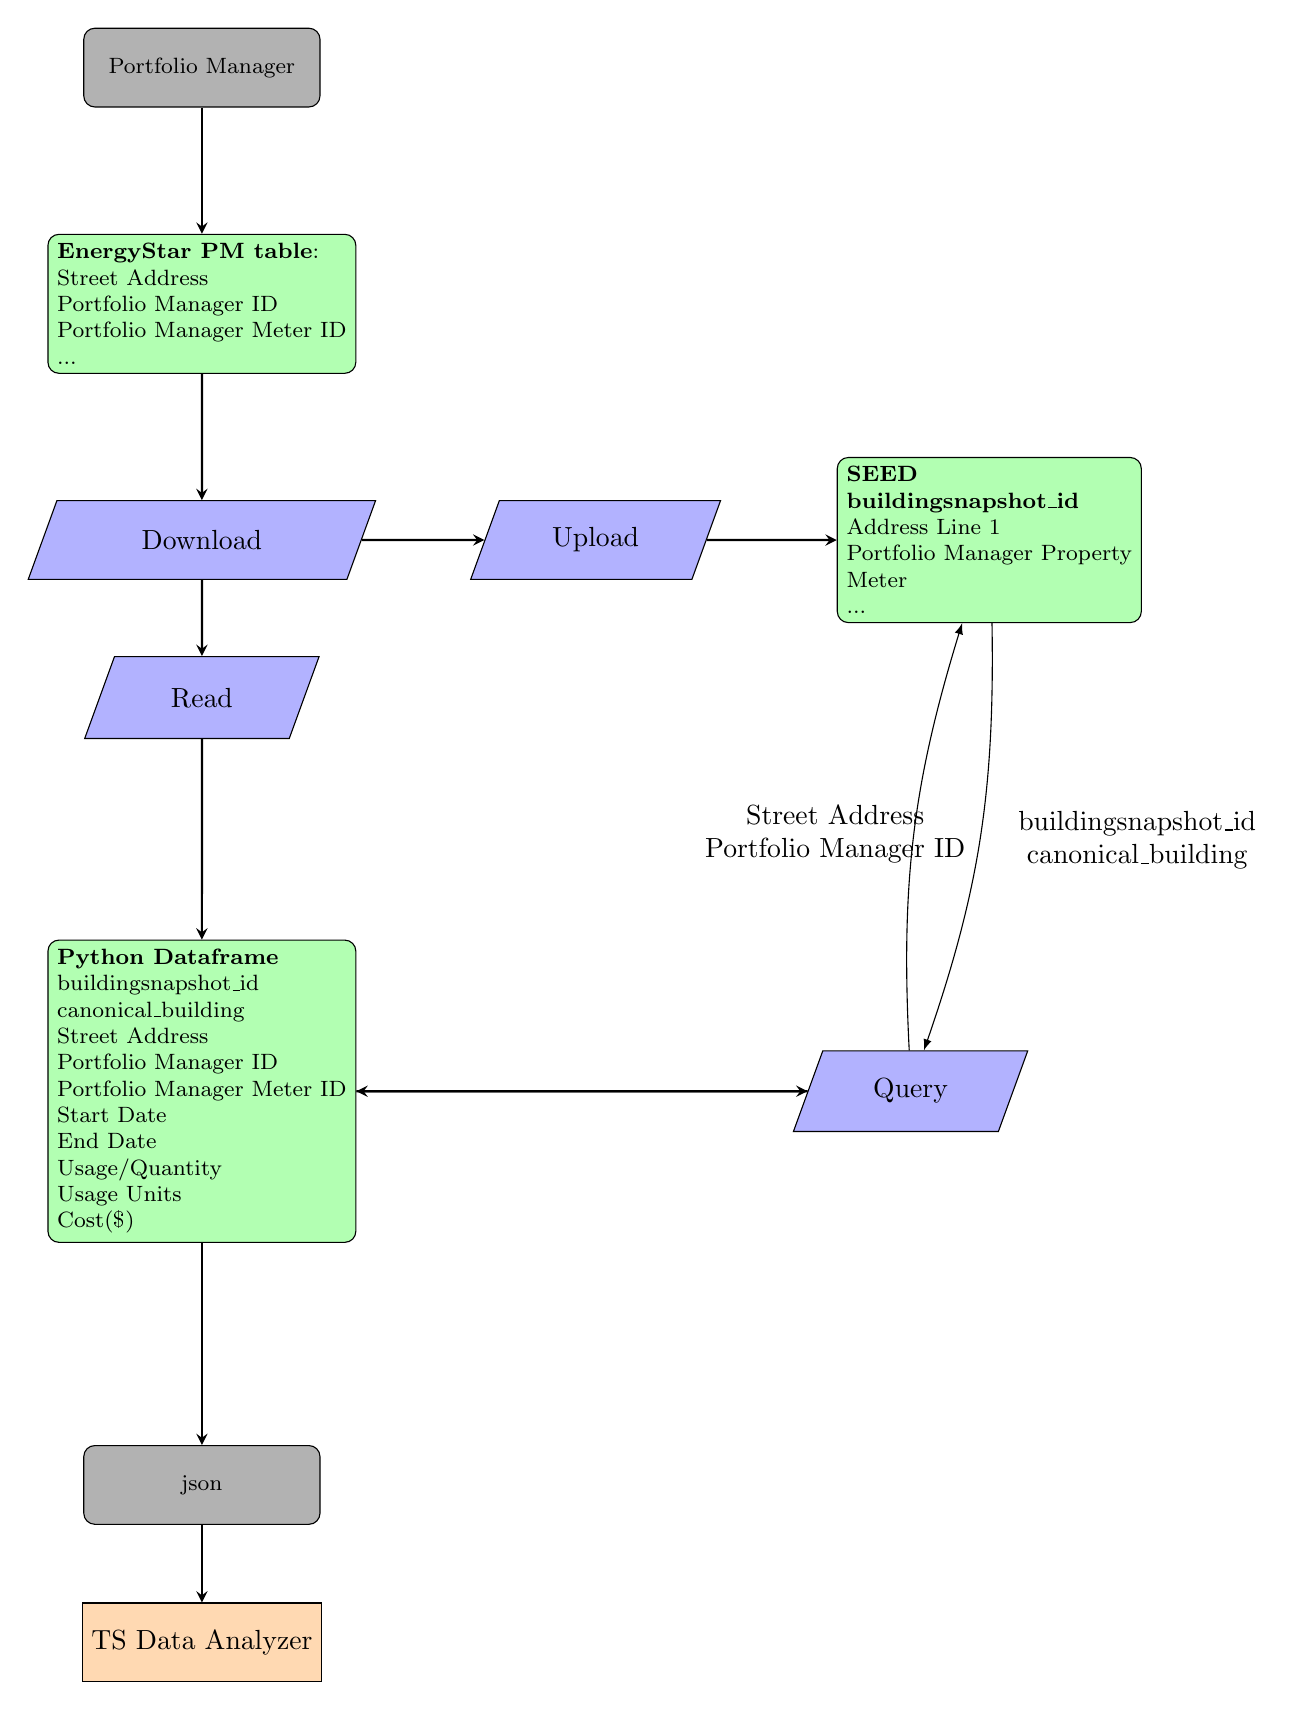
\begin{tikzpicture}
  \node (PM) [data]{Portfolio Manager};
  \node (PM_table) [database, below of=PM,yshift=-2cm]{\textbf{EnergyStar PM table}:\\
    Street Address\\
    Portfolio Manager ID\\
    Portfolio Manager Meter ID\\
    ...};
  \node(download)[query, below of=PM_table, yshift = -2cm]{Download};
  \node(upload)[query, right of=download, xshift = 4cm]{Upload};
  \node(read)[query, below of=download, yshift = -1cm]{Read};
  \node (SEED db)[database, right of = upload, xshift=4cm]{\textbf{SEED}\\
    \textbf{buildingsnapshot\_id}\\
    Address Line 1\\
    Portfolio Manager Property\\
    Meter\\
    ...};
  \node(dataframe)[database, below of=read, yshift = -4cm]{\textbf{Python Dataframe}\\
    buildingsnapshot\_id\\
    canonical\_building \\
    Street Address\\
    Portfolio Manager ID\\
    Portfolio Manager Meter ID\\
    Start Date\\
    End Date\\
    Usage/Quantity\\
    Usage Units\\
    Cost(\$)};
  \node(json)[data, below of=dataframe, yshift = -4cm]{json};
  \node(ext)[process, below of=json, yshift = -1cm]{TS Data Analyzer};
  \node(query)[query, right of=dataframe, xshift = 8cm]{Query};
  \draw[arrow](PM) -- (PM_table);
  \draw[arrow](PM_table) -- (download);
  \draw[arrow](upload) -- (SEED db);
  \draw[arrow](download) -- (read);
  \draw[arrow](download) -- (upload);
  \draw[arrow](read) -- (dataframe);
  \draw[arrow](dataframe) -- (query);
  \draw[arrow](query) -- (dataframe);
  \draw[arrow](dataframe) -- (json);
  \draw[arrow](json) -- (ext);
  %\draw[arrow, xshift = -1cm](query) -- (SEED db);
  %\draw[arrow, xshift = 1cm](SEED db) -- (query);
  \draw[-latex] (query) to[bend left=10] node [xshift=-1cm,align=center]{Street Address\\Portfolio Manager ID} (SEED
  db); 
  \draw[-latex] (SEED db) to[bend left=10] node [xshift=2cm,align=center]{buildingsnapshot\_id\\canonical\_building}
  (query);
\end{tikzpicture}

\pagebreak
\section{Discussion}
\begin{itemize}
\item Considering there might be buildings using the same address (one
  case is for \emph{maybe all buildings in CMU are entered with the
    same ``5000 Forbes Ave'' address}) choose both ``Address 1'' and
    ``Portfolio Manager ID'' for retrieving the PM ID
    (\fref{fig:dupAddressTable})
  \begin{figure}[h!]
    \centering
    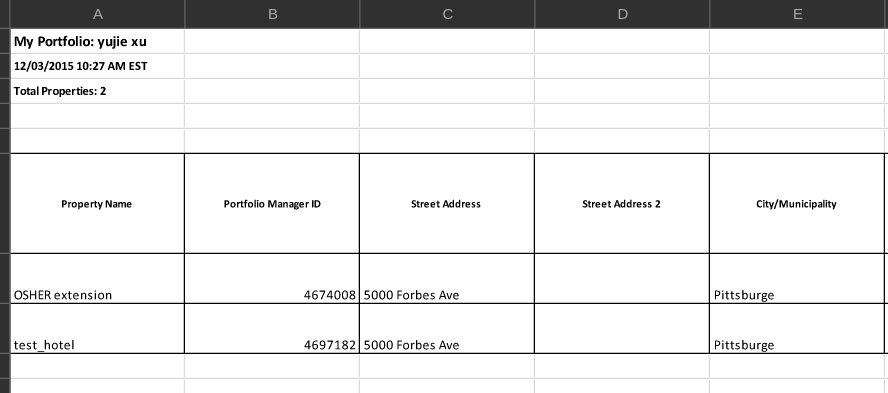
\includegraphics[width = 1.0\textwidth]{dupAddressTable.png}
    \caption{PM table that has a same address but different Portfolio
      Manager ID}
    \label{fig:dupAddressTable}
  \end{figure}
\item using ``None'' rather than ``-1'' is because of
\href{https://docs.python.org/2/library/constants.html#None}{this
  documentation}: ``None is frequently used to represent the absence
of a value''
\item \question{Is it better to directly read from PM table rather
    than create a template? because when people uploaded the table to
    PM, the ``Portfolio Manager ID'' is generate}
\end{itemize}

\newpage
\bibliographystyle{plain}
\bibliography{myCitation}
\end{document}